\section{Vector Boson Fusion}

Although the vector boson fusion (VBF) process of Higgs production has a cross section roughly ten times smaller than the production initiated by gluon-gluon interaction, the signal can be effectively obtained with few addition requirements to the event selection and with relatively low backgrounds, particularly in the fully leptonic channel.

\subsection{Selection}
The VBF topology is characterized by a pair of high energy forward-backward jets and no hadronic activity in the region between the jets. The selection involves adding the following requirements:
\begin{itemize}
\item {\bf VBF cuts: } Two leading jets with $p_T>30\:\GeVc$ satisfying
	\begin{enumerate}
	\item $\eta_1\cdot\eta_2 < 0$,
	\item $\Delta\eta > 2$,
	\item $m_{jj} > 350\:\GeVcc$,
	\item neither jet is $b$-tagged,
	\end{enumerate}
\item {\bf Central Jet Veto (CJV): } No jet with $p_T>30\:\GeVc$ between the forward-backward jets in $\eta$. 
\end{itemize}

The expected yield from Monte Carlo for a signal Higgs mass of $160\:\GeVcc$ are listed below in Table~\ref{tab:vbfyields0}.
\begin{table}[!htbp]
\begin{center}
\begin{tabular}{|c|c|c|c|c|c|}
\hline
Source & $WW$ cuts & $WW$, VBF cuts & $WW$, VBF, CJV cuts \\
\hline\hline
$t\bar{t}$ & $139.650\pm4.364$  & $10.774\pm1.212$ & $6.410\pm0.935$ \\
$t, Wt$    & $11.944\pm0.521$   & $0.888\pm0.145$  & $0.758\pm0.132$ \\
$WW$ 	   & $30.827\pm0.442$   & $3.164\pm0.140$  & $2.656\pm0.128$ \\
$WZ, ZZ$   & $5.879\pm0.213$ 	& $0.483\pm0.061$  & $0.411\pm0.057$ \\
$W+$jets   & $14.471\pm5.507$   & $0$              & $0$ \\
DY+jets    & $53.644\pm7.157$   & $6.196\pm2.651$  & $4.449\pm1.994$ \\
\hline
Background & $256.515\pm10.055$ & $21.505\pm2.923$ & $14.684\pm2.211$ \\
\hline
$ggH$ 	   & $10.768\pm0.174$ 	& $1.600\pm0.066$  & $1.380\pm0.062$ \\
\hline
$qqH$ 	   & $7.369\pm0.050$ 	& $4.953\pm0.041$  & $4.736\pm0.040$ \\
\hline
\end{tabular}
\caption{Predicted yields for $1\:\ifb$ Higgs mass of $160\:\GeVcc$.}
\label{tab:vbfyields0}
\end{center}
\end{table}

Background can be further suppressed by cutting on the dilepton mass and dilepton $\phi$-separation. The distributions for these two variables are shown in Figure~\ref{fig:vbfdilepton}. It is apparent that background can be much reduced with little loss of signal by requiring $m_{ll}<80\:\GeVcc$ and $\Delta\phi_{ll}<90\:$degrees. The expected yields after these cuts are listed in Table~\ref{tab:vbfyields1}.

\begin{figure}[!htbp]
\begin{center}
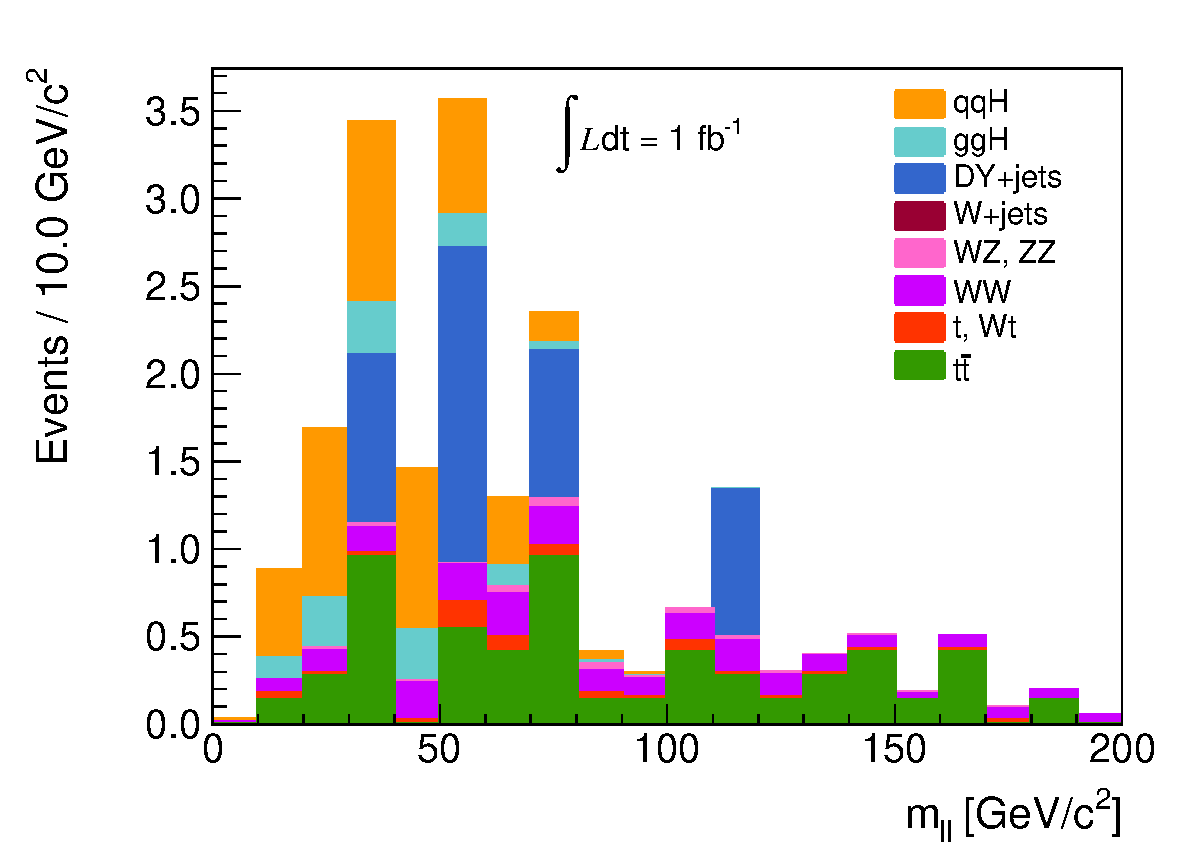
\includegraphics[scale=0.5]{figures/mll.pdf}
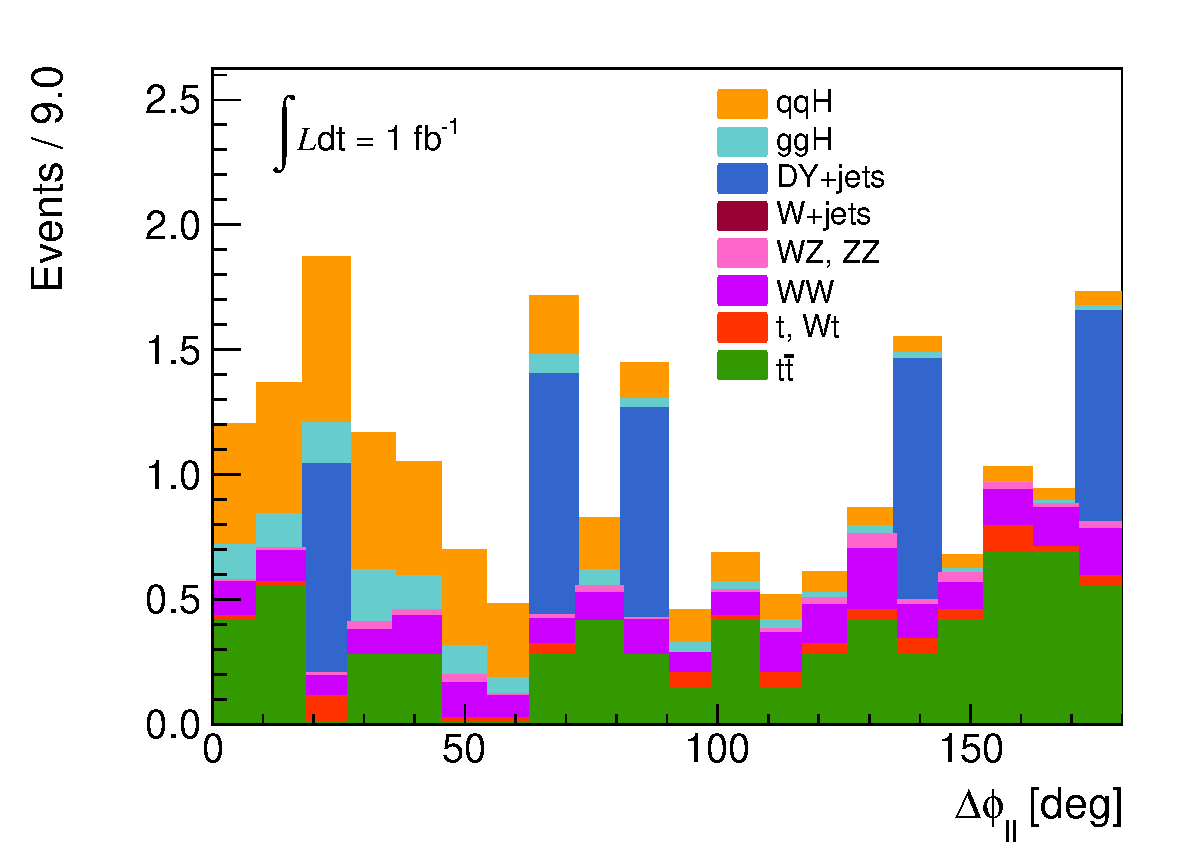
\includegraphics[scale=0.5]{figures/dphi.pdf}
\caption{Dilepton mass (top) and $\Delta\phi$ (bottom) distributions after $WW$, VBF, and CJV selection.}
\label{fig:vbfdilepton}
\end{center}
\end{figure}

\begin{table}[!htbp]
\begin{center}
\begin{tabular}{|c|c|c|}
\hline
Source & $m_{ll}<80$ & $m_{ll}<80$, $\Delta\phi_{ll}<90$ \\
\hline\hline
$t\bar{t}$ & $3.273\pm0.668$ & $1.637\pm0.472$ \\
$t, Wt$    & $0.411\pm0.099$ & $0.173\pm0.061$ \\
$WW$ 	   & $1.239\pm0.087$ & $0.811\pm0.070$ \\
$WZ, ZZ$   & $0.152\pm0.034$ & $0.106\pm0.028$ \\
$W+$jets   & $0$             & $0$ \\
DY+jets    & $3.607\pm1.808$ & $2.643\pm1.529$ \\
\hline
Background & $8.682\pm1.932$ & $5.370\pm1.603$ \\
\hline
$ggH$ 	   & $1.349\pm0.061$ & $1.133\pm0.056$ \\
\hline
$qqH$ 	   & $4.663\pm0.040$ & $3.929\pm0.037$ \\
\hline
\end{tabular}
\caption{Predicted yields for $1\:\ifb$ Higgs mass of $160\:\GeVcc$.}
\label{tab:vbfyields1}
\end{center}
\end{table}
